\documentclass[11pt,a4paper]{article}
\usepackage[utf8]{inputenc}
\usepackage{amsmath}
\usepackage{amsfonts}
\usepackage{amssymb}
\usepackage{graphicx}
\newcommand{\qed}{\hfill $\blacksquare$}
\author{Jake Bruner}
\title{Proof without words - Exploration}
\begin{document}
\maketitle
\tableofcontents
\pagebreak

\section{Introduction and Aim}

%\begin{figure}[h]
%\begin{center}
%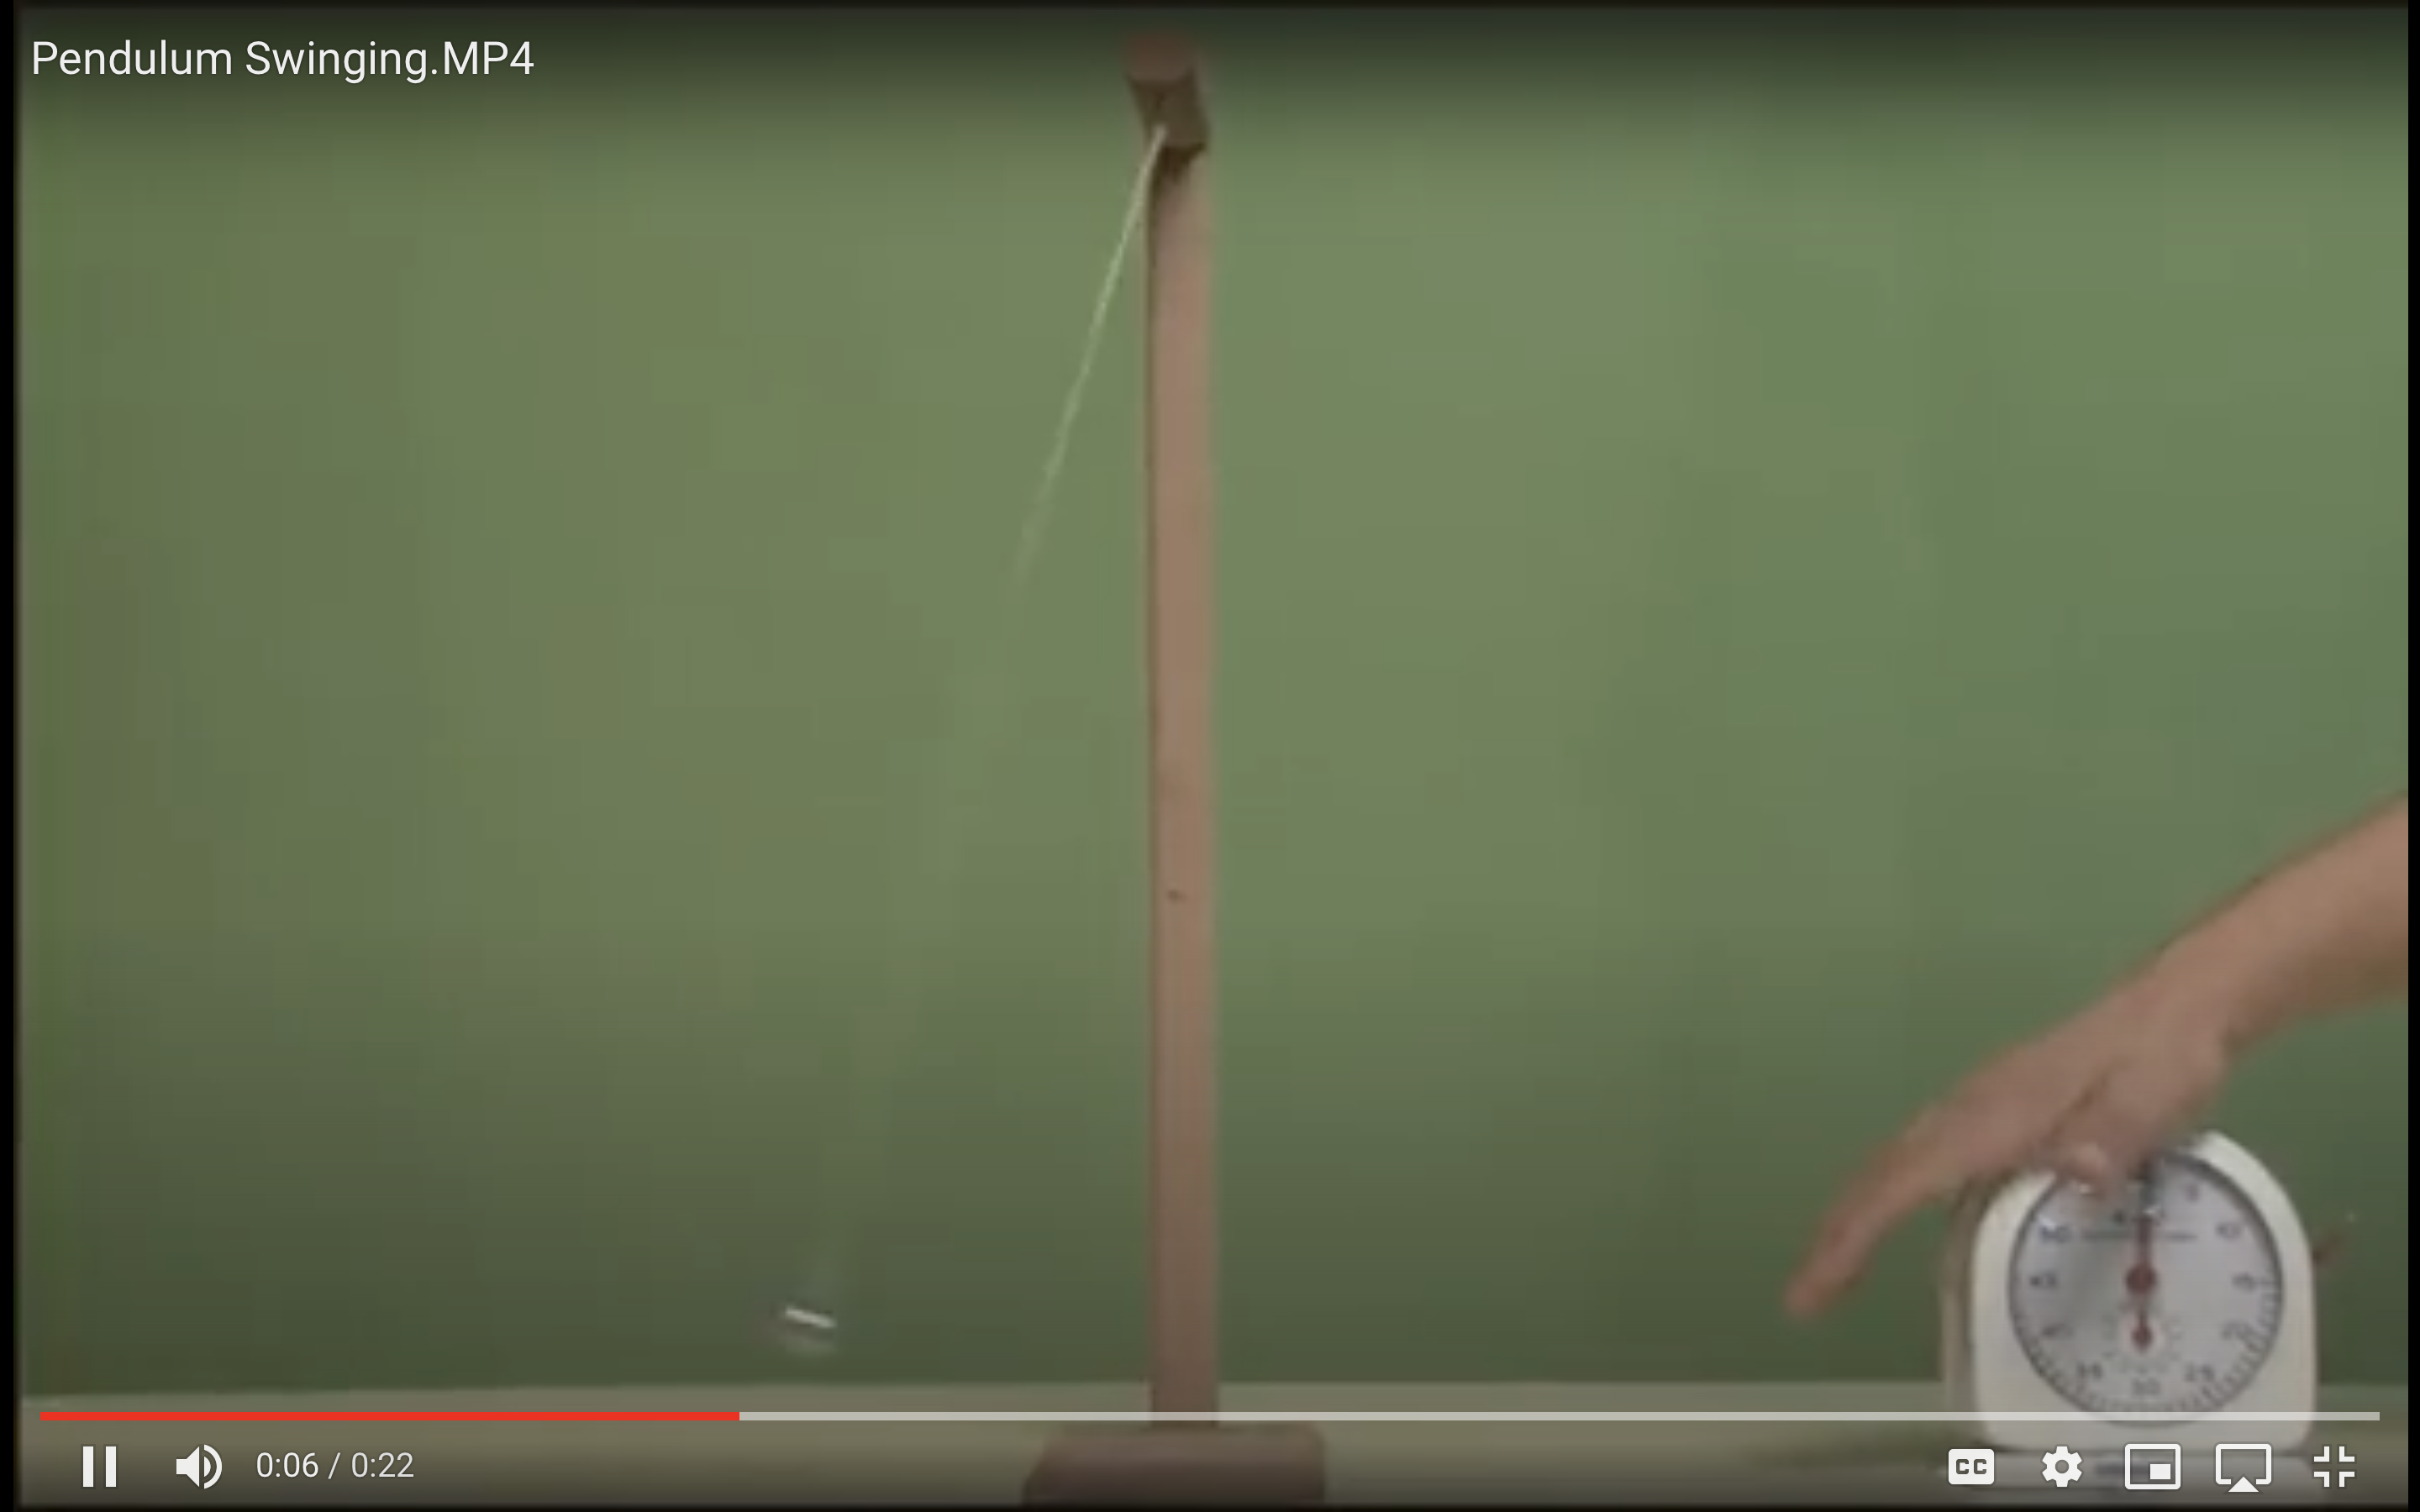
\includegraphics[scale=.24]{video.png} 
%\caption{Video Provided}
%\end{center}
%\end{figure}


respond: Do you agree with the statement “to see” is “to understand”?




\section{Understanding Proof Through Pythagorean Theorem}
\subsection{The First Proof \textit{circa} 200 BCE}
\subsection{Comparison to Modern Methods}
compare to contradiction proof
discuss proofs in class
\subsection{Are Proofs-Without-Words Proofs?}
quote nelson 
discuss the questionjjj
\subsection{Exemplifying Wordless Proof}
choose another proof from book
\pagebreak
\section{When Visual Proof Becomes Hectic}

Consider Richard Courant's proof of integration by parts: 

\begin{figure}[h]
\begin{center}
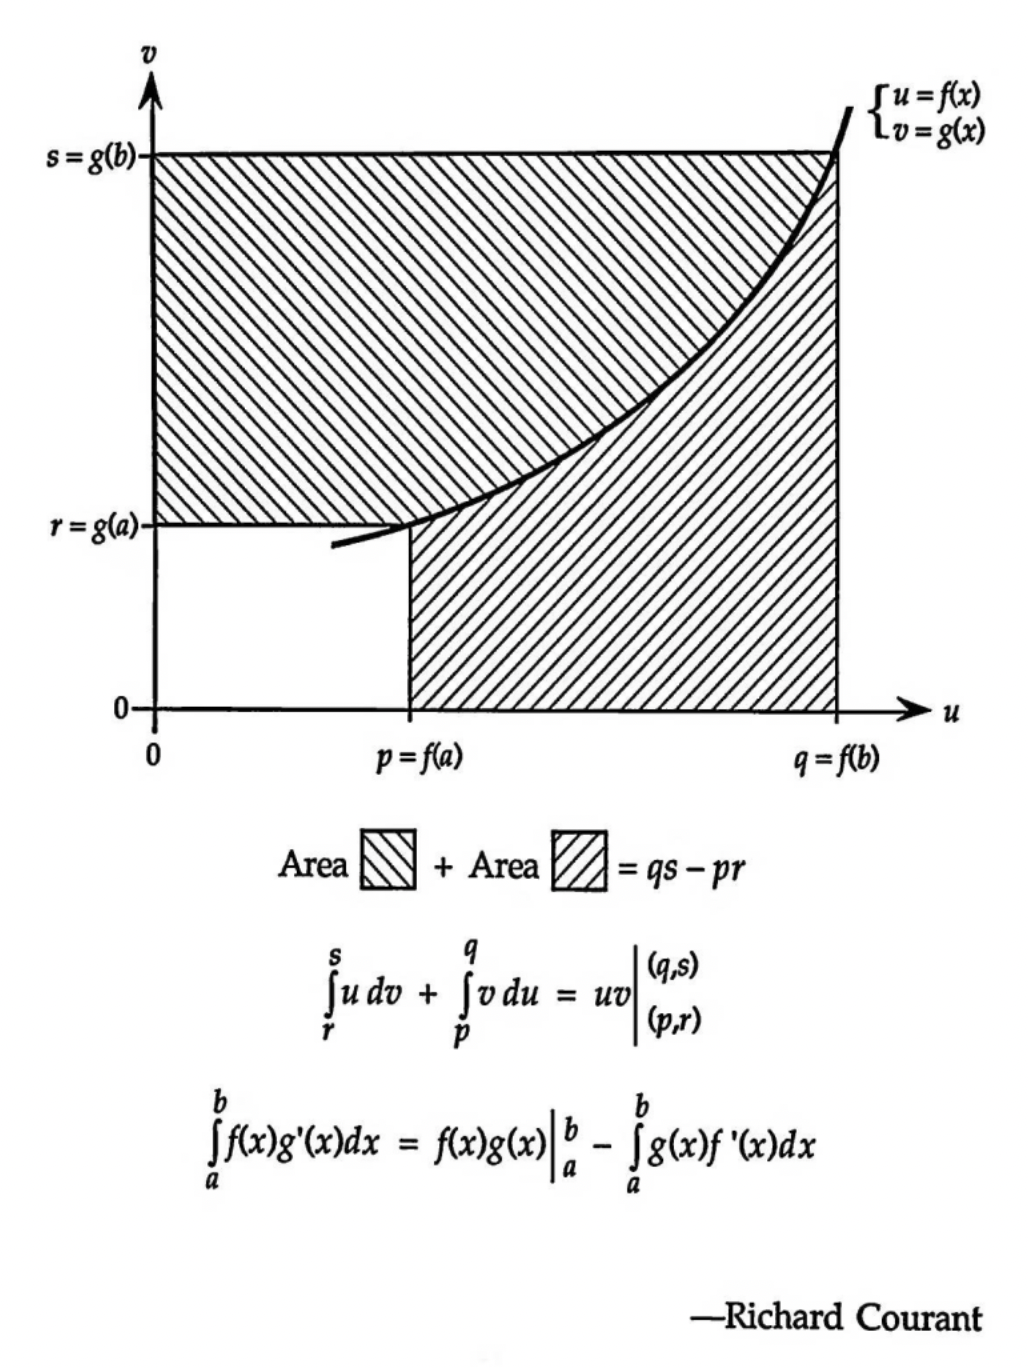
\includegraphics[scale=.5]{proof of ibp} 
\end{center}
\end{figure}

This proof--although rigorous--is an extremely confusing jumble of variables upon first glance.  Without text to aid, a few key assumptions are not immediately obvious. For instance, Courant's proof includes that the curve is bound by the parametric equation, $ \big( f(x), \ g(x) \big) $, made worse by the fact $x$ is the parameterising variable.  Furthermore, this 'visual' proof either requires the reader to figure out or have prior knowledge of how to integrate a parametric curve. Overall, the beauty of this proof cannot be realised without close examination, which detracts from its accessibility.
\pagebreak

Attempting to depict this proof in a more straight-forward way, it might be useful to relabel the axis and variables to be more friendly to math conventions. \\
\begin{figure}[h]
\begin{center}
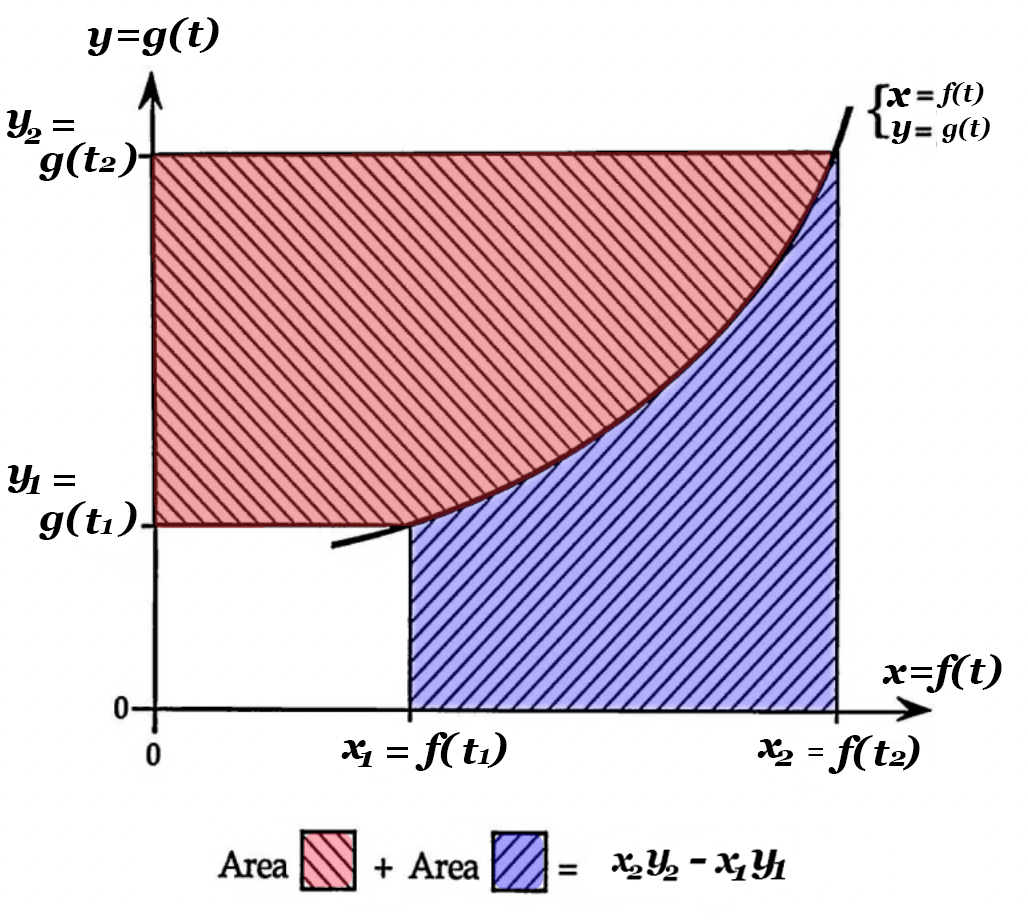
\includegraphics[scale=.4]{modified proof of ibp} 
\end{center}
\end{figure} \\
Breaking this down piece by piece, it's initially helpful to reiterate these parametric equations in terms of non-parametric functions so that integration and derivation are more explicit. Parametric curves are easier to digest conceptually when they are discussed in reference to the path a vector draws. In this example, it is possible to imagine a 2d vector with $x$ component $f(t)$ and $y$ component $g(t)$.  As the variable $t$ sweeps through inputs (for example, time increasing from zero continuously) the output/head of the vector will draw out a continuous curve. So clearly here,  $y$ is a function of $x$ (even if its not explicitly--or technically implicitly--defined since $y$ varies according to whatever value $x$ takes on) and vice-versa.
\begin{align*}
x(y) &= x = f(t)\\
y(x) &= y = g(t)
\end{align*}
Given that these variables simply correspond to the x and y axis, it is possible to understand these integrals without knowing the process for parametric curves. Simply put, if one knows that an area under a curve can be represented by an integral with respect to the axis variable (usually $x$), it should logically be a similar process to see the area bounded by the vertical axis.  For the x axis, the area in the blue is simply:
\begin{align*}
A_b = \int_{x_1}^{x_2} y\ dx
\end{align*}
Now, the area bound by the curve and the y-axis takes the same form.  Although, for many this seems like sacrilege, this idea is perfectly legal; one can imagine this as defining the horizontal axis as $y$ and the vertical axis as $x$ then finding the area under a curve.  So hence, the area in red is simply:
\begin{align*}
A_r = \int_{y_1}^{y_2} x \ dy
\end{align*}
Now, the sum of these two integrals would represent the total area of the rectangular section of the graph,  minus the area in the white. Again,  the total area $A_b + A_r$ is equal to the large rectangle $x_2 \times y_2$ minus the small, white rectangle $x_1 \times y_1$.
\begin{align*}
A_b &+ &A_r &= &large\ rectangle\ &- &small\ rectangle \\
\int_{x_1}^{x_2} y \ dx &+ &\int_{y_1}^{y_2} x \ dy &= &( x_2 \times y_2)\ \ & - &(x_1 \times y_1)
\end{align*}
From here, its helpful to write the subtraction of the two areas as a product of the axis variables $x$ and $y$ evaluated at the same bounds as the integral. This can be thought as similar to the reverse process of evaluating a definite integral. It might be unclear how the equation $x \cdot y(x)$ could be evaluated for $x_1 ,\ x_2$, since the function $y(x)$ has not been defined. Since $y$ varies with $x$ (for any parametric curve), it is formally possible to implicitize 
\begin{align*}
xy \Big|_{x_1}^{x_2} =  x_2 y_2\ -\ & x_1 y_1
\end{align*}
and
\begin{align*}
yx \Big|_{y_1}^{y_2} =  x_2 y_2\ -\ & x_1 y_1
\end{align*}
\textit{(This makes even more sense when the functions are written explicitly.)} So substituting this simplification into the original equation:
\begin{align*}
\int_{x_1}^{x_2} y \ dx + \int_{y_1}^{y_2} x \ dy &= xy \Big|_{x_1}^{x_2} = yx \Big|_{y_1}^{y_2} 
\end{align*}
Rewritten in function notation:
\begin{align*}
\int_{x_1}^{x_2} y(x) \ dx + \int_{y_1}^{y_2} x(y) \ dy &= x \cdot y(x) \Big|_{x_1}^{x_2} = y\cdot x(y) \Big|_{y_1}^{y_2}
\end{align*}
The most conceptually foreign step is now converting all these bounds and function variables into the parametric variable $t$.  Since the functions $x$ and $y$ are defined in terms of the functions $f(t)$ and $g(t)$,  its possible to define $x$ as a function of $t$ instead of a function of $y$ (and vice-versa) to eliminate the self-referential and self-inverse confusion.  So hence, rewritten in terms of t:
\begin{align*}
\int_{t_1}^{t_2} y(t) \ dx(t) + \int_{t_1}^{t_2} x(t) \ dy(t) = x(t)\cdot y(t) \Big|_{t_1}^{t_2} 
\end{align*}
Rearranging we get the a form of integration by parts, given that: \begin{align*}
d\big( y(t) \big) &= y'(t)\ dt \\
d\big(x(t)\big) &= x'(t)\ dt:
\end{align*}
Hence:
\begin{align*}
\int_{t_1}^{t_2} x(t) \ d\big(y(t)\big) = x(t)y(t) \Big|_{t_1}^{t_2} \ - \int_{t_1}^{t_2} y(t) \ d\big(x(t)\big)
\end{align*}
Or sometimes written as:
\begin{align*}
\int_{t_1}^{t_2} x(t)y'(t) \ dt = x(t)y(t) \Big|_{t_1}^{t_2} \ - \int_{t_1}^{t_2} y(t)x'(t)\ dt
\end{align*}
Rewritten with indefinite integrals, it is also:
\begin{align*}
\int x\ dy = xy \ - \int y \ dx 
\end{align*}
\qed

\section{Conclusion}


\end{document}
